\documentclass[pdftex,letterpaper,11pt]{article}

%%
%%  Graphics packages
%%
\pdfoutput=1
\usepackage[dvips,pdftex]{graphicx,color}  %%  allow colored text
\usepackage{array}
\usepackage{epstopdf}  %%  convert EPS --> PDF
\usepackage[tableposition=top]{caption}
\usepackage{wrapfig}
%%
%%  Math/Symbol packages
%%
\usepackage{amsmath}   %%  contains advanced math extensions
\usepackage{latexsym}  %%  adds other symbols in to be used in math mode
\usepackage{amssymb}   %%  adds new symbols in to be used in math mode
\usepackage[utf8]{inputenc}  %%  Use UTF-8 encoding
%%
%%  Bibliography packages
%%
%%  \citep{} --> [Wilson et al., YYYY]
%%  \citet{} --> Wilson et al., [YYYY]
\usepackage[square,authoryear,compress]{natbib}
%%
%%  Color packages
%%
\usepackage{color}
\usepackage[rgb,dvipsnames]{xcolor}
%%
%%  Referencing packages
%%
\usepackage{hyperref}     %%  Allow internal and external references
%%  Setup hyper references
%%    colorlinks, urlcolor, citecolor, and linkcolor --> define appearance of links
%%    the rest --> define options for the PDF viewer when opened
\hypersetup{colorlinks=true, urlcolor=blue, citecolor=black, linkcolor=black, bookmarksopen=true, bookmarks=true, pdftoolbar=true, pdfmenubar=true, bookmarksopenlevel=\maxdimen, pdftex, bookmarksnumbered=true, bookmarkstype=toc, debug=true}
%%
%%  Page Formatting packages
%%
\usepackage{titlesec}     %%  Allows use of \titleformat and \titlespacing
%%  Define page size and margin sizes
\usepackage[top=1.0in, bottom=1.0in, left=0.875in, right=0.875in]{geometry}
\usepackage{setspace}
\linespread{1.00}         %%  Set line spacing to single space
\usepackage{indentfirst}  %%  Force first paragraph to indent
\usepackage{fancyhdr}     %%  Allow the use of custom headers and footers
%%
%%  Extra Formatting packages
%%
\usepackage{tocloft}      %%  Allow the user to format the Table of Contents
\usepackage{lastpage}     %%  Allow user to know total # of pages (e.g. page 5 of 9)

%%
%%  Dummy text production packages
%%
\usepackage[english]{babel}
%%    Commands:
%%      \blindlist{env}[n]
%%      \blindtext[n]
%%      \blinditemize[n]
%%      \blindenumerate[n]
%%      \blinddescription[n]
%%      \blindmathtrue
%%      \blindmathfalse
%%
%%    Input Definitions:
%%         env = environment to use [e.g., itemize, enumerate, or description]
%%         n   = # of paragraphs to print
\usepackage[math]{blindtext}

%%  Define the color grey
\definecolor{grey}{gray}{0.7}

%%########################################################################################
%%  Page Size and Formatting Settings
%%########################################################################################
\special{papersize=8.5in,11in}  %%  Define total useable area
\setlength{\textwidth}{6.5in}   %%  Define width of useable area
\setlength{\textheight}{9.0in}  %%  Define height of useable area
%%  -> Define the margin sizes
\setlength{\oddsidemargin}{0.0cm}
\setlength{\evensidemargin}{0.0cm}
\setlength{\topmargin}{-0.50in}
\setlength{\hoffset}{-0.125in}
%%  -> Define the header and footer sizes
\setlength{\headheight}{0.2in}
\setlength{\headsep}{0.25in}
\setlength{\footskip}{0.35in}
%%  -> Define horizontal width of header&footer
\setlength{\headwidth}{1.00\textwidth}
%%  Adjust spacing above/below captions
\setlength{\abovecaptionskip}{5pt}
\setlength{\belowcaptionskip}{1pt}
%%  Adjust spacing between last top float or first bottom float and the text
\setlength{\textfloatsep}{2pt}
%%  Adjust spacing before/after an in-text float
\setlength{\intextsep}{2pt}
%%  Adjust spacing between lines in text
\setlength{\parskip}{0pt}
%%  Adjust spacing before/after a paragraph in each item in enumerate
\setlength{\parsep}{-2pt}
%%  Adjust spacing before/after each item in enumerate
\setlength{\itemsep}{-2pt}
%%  Adjust spacing before an enumerate environment
\setlength{\topsep}{-2pt plus 1pt minus 1pt}

%%########################################################################################
%%  Table of Contents (ToC) Formatting Settings
%%########################################################################################
%%  Adjust space between lines in TOC
\setlength{\cftbeforesecskip}{-1pt}         %%  Section spacing
\setlength{\cftbeforesubsecskip}{-2pt}      %%  Subsection
\setlength{\cftbeforesubsubsecskip}{-2pt}   %%  Subsubsection
%%  Adjust font size in ToC
\renewcommand{\cftsecfont}{\normalsize\bfseries}
\renewcommand{\cftsubsecfont}{\small}
\renewcommand{\cftsubsubsecfont}{\footnotesize}
%%  Define # of levels labeled in TOCs
%%    1  =  show down to Sections
%%    2  =  show down to Subsections
%%    3  =  show down to Subsubsections
\setcounter{tocdepth}{3}

%%  Define new ToC section name
\renewcommand{\cftmarktoc}{{\bf \Large Table of Contents}}
%%  Define new List of Tables section name
\renewcommand{\cftmarklot}{{\bf \Large List of Tables}}
%%  Define new List of Figures section name
\renewcommand{\cftmarklof}{{\bf \Large List of Figures}}

%%  Define new prefix labels in the List of Tables and Figures
%\renewcommand{\cftfigpresnum}{Figure }
%\renewcommand{\cfttabpresnum}{Table }

%%########################################################################################
%%  Section Formatting options
%%########################################################################################
%%  \titleformat{<command>}[<shape>]{<format>}{<label>}{<sep>}{<before>}[<after>]
%%     (1 em = N points, where N = font size
%%       [e.g., 1 em = 10 pt for 10 pt font ])
\titleformat{\section}[hang]{\Large\bfseries}{\thesection}{10pt}{}  %% horizontal spacing
\titleformat{\subsection}[hang]{\large\bfseries}{\thesubsection}{7pt}{}
\titleformat{\subsubsection}[hang]{\normalsize\bfseries}{\thesubsubsection}{5pt}{}

%%########################################################################################
%%  Headers and Footers
%%########################################################################################
%%  -> Define the short title
\newcommand{\shorttitle}{This is my short title}
%%  -> Define the footer note
\newcommand{\ftrnote}{\textcolor{grey}{\emph{PONTIFICATING EXAMPLES}}}
%%  -> Define the headers [Left, Center, Right]
\lhead[\it \shorttitle ]{\it \shorttitle}
\chead[]{}
\rhead[ \thepage\ of \pageref{LastPage} ]{ \thepage\ of \pageref{LastPage} }
%%  -> Define the footers [Left, Center, Right]
\lfoot[]{}
\cfoot[\ftrnote]{\ftrnote}
\rfoot[]{}
%%  -> Define line thickness for header/footer lines
\renewcommand{\headrulewidth}{0.5mm}  %%  set to 0mm if no line desired
\renewcommand{\footrulewidth}{0.5mm}
%%  -> Change header/footer line color to teal
%%     Header Line
\renewcommand{\headrule}{{\color{teal}\hrule width\headwidth height\headrulewidth \vskip-\headrulewidth}}
%%     Footer Line
\renewcommand{\footrule}{{\color{teal}\vskip-\footruleskip\vskip-\footrulewidth
\hrule width\headwidth height\footrulewidth\vskip\footruleskip}}
%%  -> Set the page style to use these custom headers/footers
\pagestyle{fancy}

%%########################################################################################
%%  Change Table and Figure Labels
%%########################################################################################
%%  Change Figure counters to S1, S2, ..., SN
\renewcommand{\thefigure}{S\arabic{figure}}
%%  Change Table counters to I, II, III, ...
\renewcommand{\thetable}{\Roman{table}}
%%########################################################################################
%%  Footnotes
%%########################################################################################
%%  Change footnote marks from symbol to numbers
\makeatletter  %%  Allow the use of @-symbol in the followin TeX definition
\let\@fnsymbol\@arabic
\makeatother   %%  Shut-off @-symbol functionality
%%  Change footnote marks
\renewcommand{\thefootnote}{\arabic{footnote}}


%%########################################################################################
%%%%######################################################################################
%%%%%%####################################################################################
%%%%%%%%  Begin the document
%%%%%%####################################################################################
%%%%######################################################################################
%%########################################################################################
\begin{document}
%%  Define style of bibliography
\bibliographystyle{agu08}  %%  agu08.bst is distributed by AGU

%%
%%       \titlespacing{ command }{ left }{ before }{ after }[ right ]
%%         before = X plus Y minus Z
%%           => This means that:
%%                X  =  value we would like
%%                Y  =  max value TeX can increase X
%%                Z  =  max value TeX can decrease X
%%
%%  -> Define spacing for floats
\titlespacing{\enumerate}{0pt}{0pt plus 1pt minus 1pt}{0pt plus 1pt minus 1pt}
\titlespacing{\figure}{0pt}{0pt plus 1pt minus 1pt}{0pt plus 1pt minus 1pt}
\titlespacing{\table}{0pt}{0pt plus 1pt minus 1pt}{0pt plus 1pt minus 1pt}
\titlespacing{\threeparttable}{0pt}{0pt plus 1pt minus 1pt}{0pt plus 1pt minus 1pt}
\titlespacing{\tablenotes}{0pt}{0pt plus 1pt minus 1pt}{0pt plus 1pt minus 1pt}
\titlespacing{\wrapfigure}{0pt}{0pt plus 1pt minus 1pt}{0pt plus 1pt minus 1pt}
%%  -> Define spacing for sections
\titlespacing{\section}{0pt}{3pt plus 2pt minus 2pt}{3pt plus 2pt minus 2pt}
\titlespacing{\subsection}{0pt}{2pt plus 2pt minus 2pt}{2pt plus 2pt minus 2pt}
\titlespacing{\subsubsection}{0pt}{1pt plus 2pt minus 2pt}{1pt plus 2pt minus 2pt}

%%
%%  Format Table/Figure captions
%%
\captionsetup[table]{font=large,position=above,justification=centering}
\captionsetup[wrapfigure]{figurename=FIG.,labelfont=bf,skip=5pt,font=footnotesize,justification=RaggedRight}
%\captionsetup[figure]{figurename=FIG.,skip=1pt,font=footnotesize,position=below,justification=RaggedRight,labelsep=vline}
%%----------------------------------------------------------------------------------------
%%  Title Page
%%----------------------------------------------------------------------------------------
%%  Page Format and Numbering
\pagestyle{plain}
\pagenumbering{arabic}
%%  Define Title
\title{\bf Title:  Some Useful Preamble Examples}
%%  Define Author
\author{Author:  Pontificating Blowhard}
%%  Define current date
\date{\today}
\maketitle  %%  necessary to make LaTeX print title

%%  Shut off page numbering here
\thispagestyle{empty}
\clearpage
%%----------------------------------------------------------------------------------------
%%  Auto-generated Table of Contents (ToC)
%%----------------------------------------------------------------------------------------
%%  Shut off default ToC section name
\renewcommand{\contentsname}{}
\tableofcontents  %%  Output ToC

%%  Shut off page numbering here
\thispagestyle{empty}
\clearpage
%%----------------------------------------------------------------------------------------
%%  Auto-generated List of Tables
%%----------------------------------------------------------------------------------------
%%  Shut off default List of Tables section name
\renewcommand{\listtablename}{}
\listoftables     %%  Output List of Tables

%%  Shut off page numbering here
\thispagestyle{empty}
\clearpage
%%----------------------------------------------------------------------------------------
%%  Auto-generated List of Figure
%%----------------------------------------------------------------------------------------
%%  Shut off default List of Figure section name
\renewcommand{\listfigurename}{}
\listoffigures     %%  Output List of Figure

%%  Shut off page numbering here
\thispagestyle{empty}
\clearpage

%%  -> Set the page style to use these custom headers/footers
\pagestyle{fancy}
\pagenumbering{arabic}  %%  start page numbering here
\setcounter{page}{1}    %%  set page number to 1
\blindmathfalse
%%----------------------------------------------------------------------------------------
%%  Section:  First Section
%%----------------------------------------------------------------------------------------
\section{\label{sec:First}First Section}
\indent  \textbf{\textcolor{Red}{\blindtext[1]}}\footnote{ See awesome webpage at:  \href{http://tetra.space.umn.edu/wiki/doku.php/latex}{Awesome} }

\clearpage
%%----------------------------------------------------------------------------------------
%%  Section:  Second Section
%%----------------------------------------------------------------------------------------
\section{\label{sec:Second}Second Section}
\indent  \textbf{\textcolor{Purple}{\blindtext[2]}}
%%----------------------------------------------------------------------------------------
%%  Subsection:  First Subsection
%%----------------------------------------------------------------------------------------
\subsection{\label{subsec:First}First Subsection}
\indent  \textbf{\textcolor{Gray}{\blindtext[1]}}
%%----------------------------------------------------------------------------------------
%%  Subsubsection:  First Subsubsection
%%----------------------------------------------------------------------------------------
\subsubsection{\label{subsubsec:First}First Subsubsection}
\indent  \textbf{\textcolor{Orange}{\blindtext[1]}}


\clearpage
%%----------------------------------------------------------------------------------------
%%  Section:  Math Section
%%----------------------------------------------------------------------------------------
\section{\label{sec:Math}Math Section}

\blindmathtrue
\indent  \blindtext[1]
\blindmathfalse

\clearpage
%%----------------------------------------------------------------------------------------
%%  Section:  Figure Section
%%----------------------------------------------------------------------------------------
\section{\label{sec:Figure}Figure Section}
\indent  \blindtext[1]

%%++++++++++++++++++++++++++++++++++++++++++++++++++++++++++++++++++++++++++++++++++++++++
%% Image:  Nonlinear Wave Steepening
%%++++++++++++++++++++++++++++++++++++++++++++++++++++++++++++++++++++++++++++++++++++++++
\begin{wrapfigure}[17]{r}{0.5\textwidth}
  \centering
    {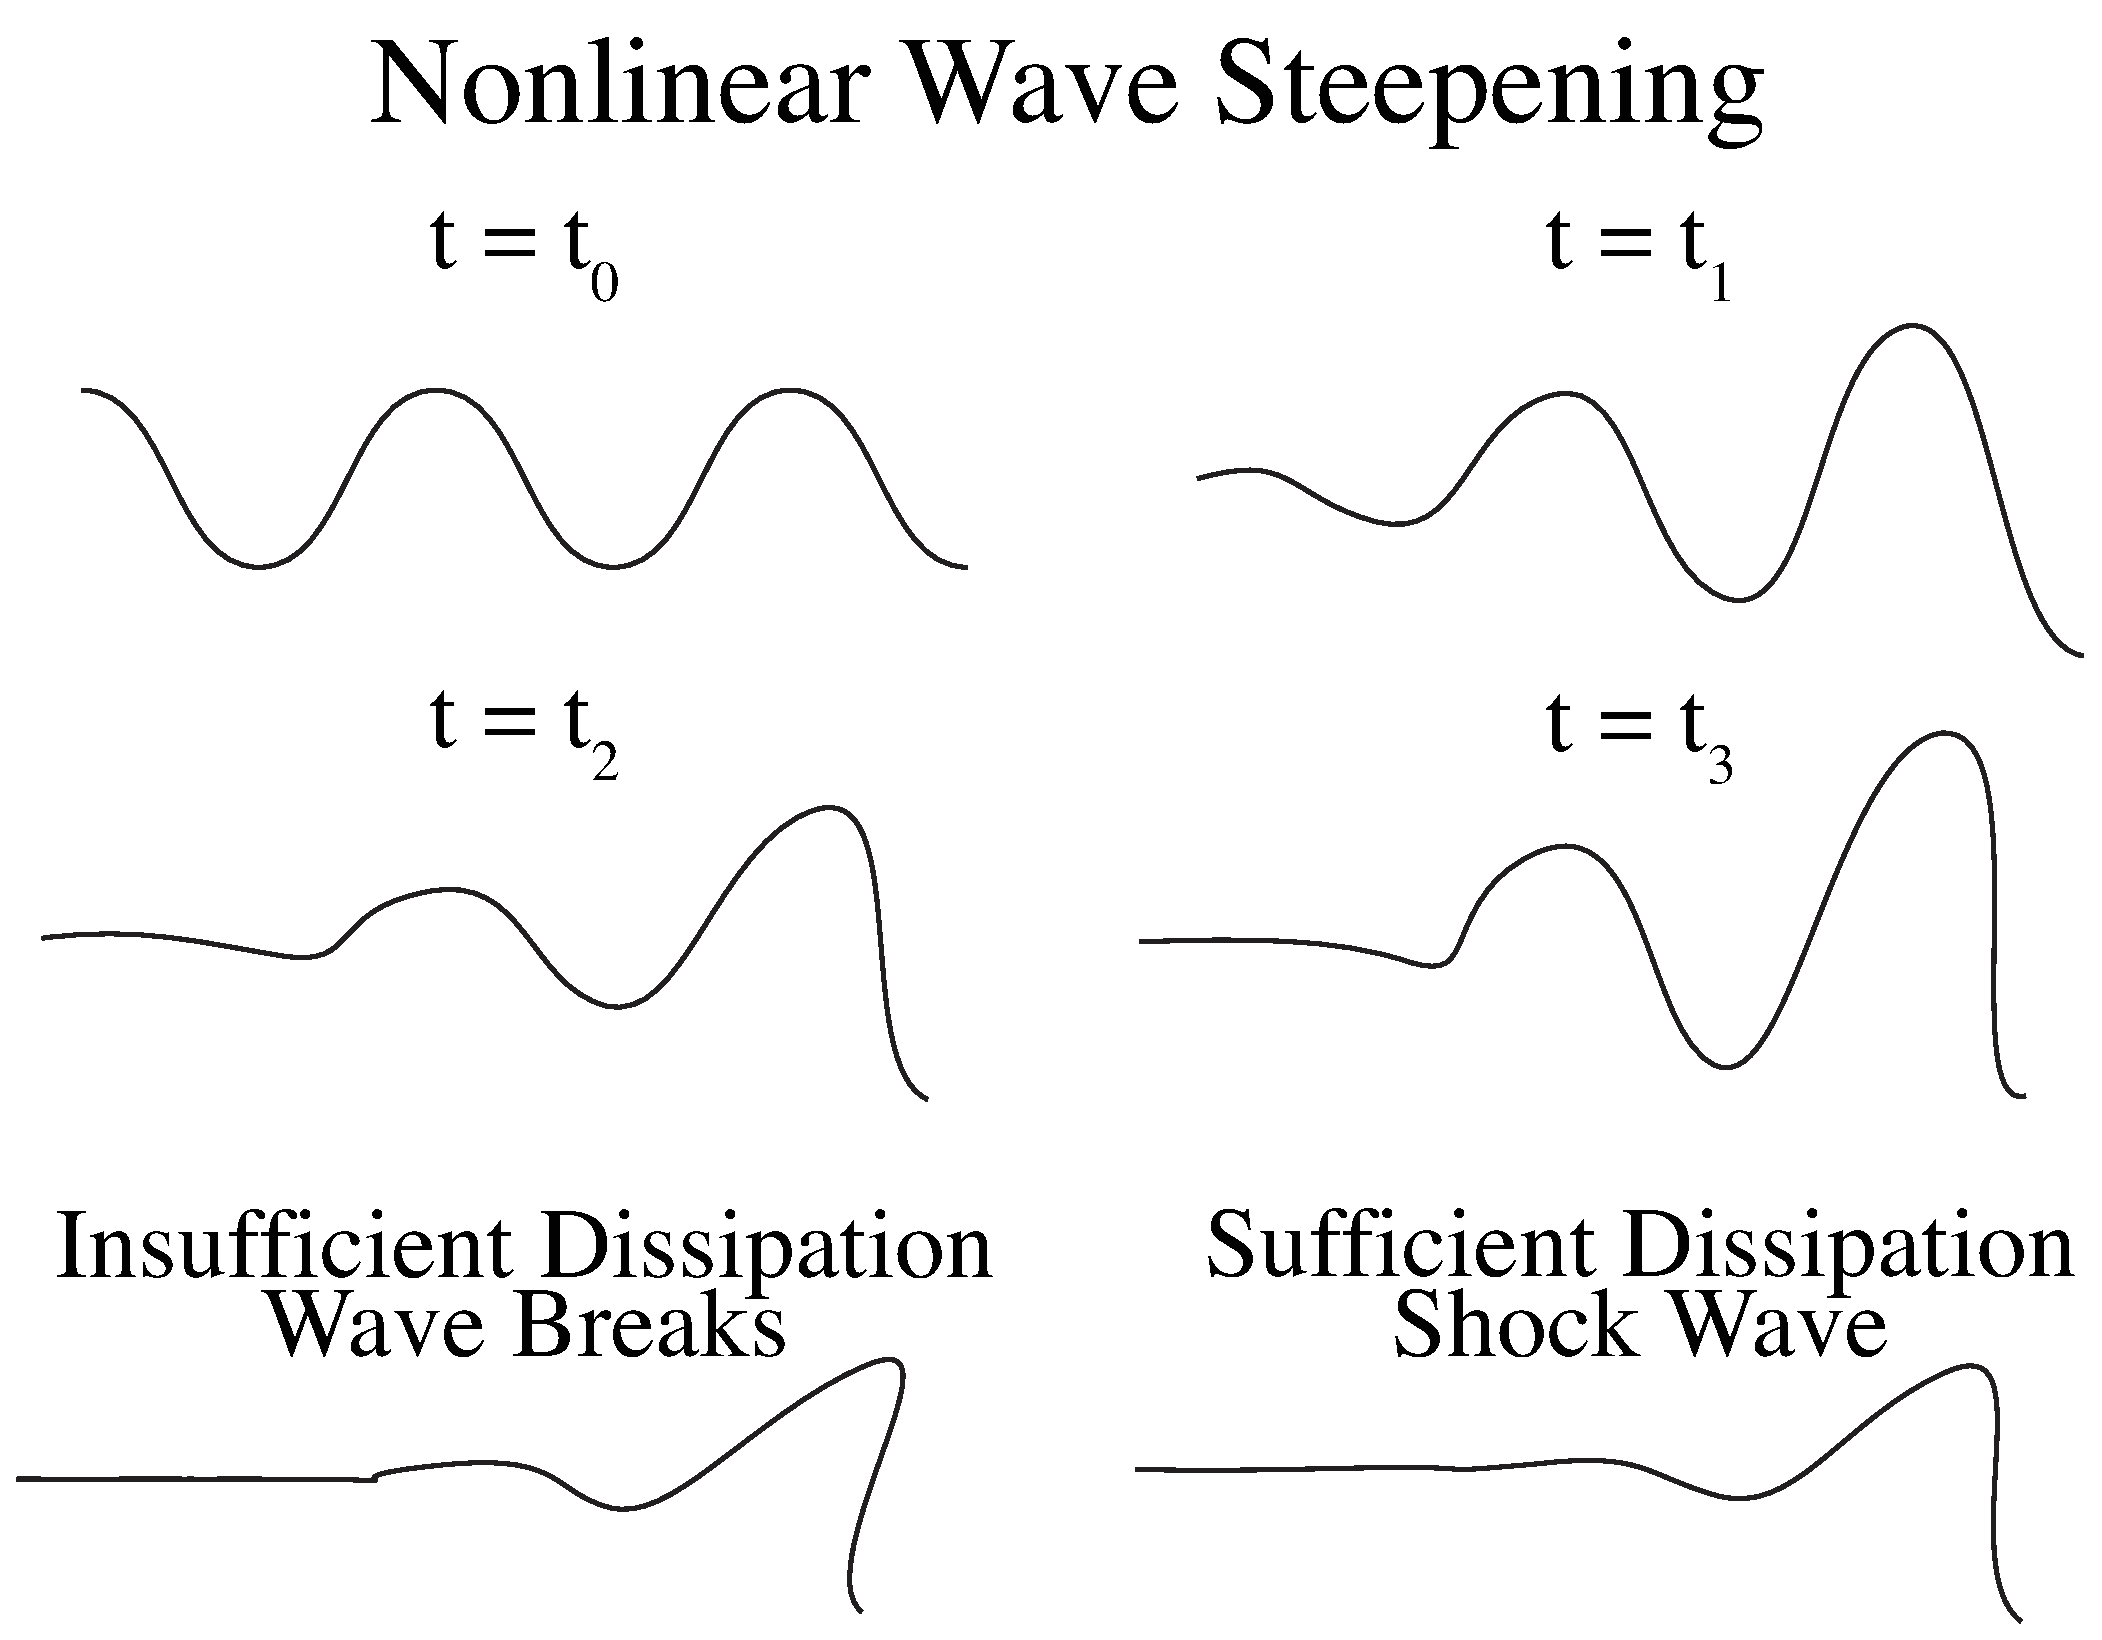
\includegraphics[trim = 0mm 0mm 0mm 0mm, clip, width=0.45\textwidth]
    {NonlinearWaveSteepening}}
    %%  Define caption
    \caption[Nonlinear Wave Steepening]{Figure illustrating how larger amplitude waves can catch smaller amplitude waves and eventually overrun (wave breaking) or match (stable discontinuity) their position.}
    \label{fig:nonlinear}
\end{wrapfigure}
%%++++++++++++++++++++++++++++++++++++++++++++++++++++++++++++++++++++++++++++++++++++++++
%% Image:  Nonlinear Wave Steepening
%%++++++++++++++++++++++++++++++++++++++++++++++++++++++++++++++++++++++++++++++++++++++++

\indent  \blindtext[2]

\indent  \blindtext[1]

\clearpage
%%----------------------------------------------------------------------------------------
%%  Section:  Special Characters Section
%%----------------------------------------------------------------------------------------
\section{\label{sec:Special}Special Characters Section}
\indent  In this section I provide a few examples of how to typeset special characters.  You may need to use the \textbf{\textit{inputenc}} package with the option \textit{utf8} set.  \footnote{If you examine the source file (\textbf{\textit{useful\_examples.tex}}) for this PDF file, you will see an example of how to create a table.}

%%========================================================================================
%%  Table:  Special Characters
%%========================================================================================
\begin{table}[htb]
  \centering
  \caption[Special Character Commands]{Special Character Commands in Text and Math Mode}
  \label{tab:specialtext}
    \begin{tabular}{| c | c | c | c | c |}
      \hline
      \textbf{Text}    & \textbf{Math}    & \textbf{Text}   & \textbf{Math}   & \textbf{Description} \\
      \textbf{Command} & \textbf{Command} & \textbf{Result} & \textbf{Result} & \\
      \hline
      \verb+\`{o}+     &   \verb+\grave{o}+   &  \`{o} &   $\grave{o}$   & grave accent \\
      \verb+\'{o}+     &   \verb+\acute{o}+   &  \'{o} &   $\acute{o}$   & acute accent \\
      \verb+\^{o}+     &    \verb+\hat{o}+    &  \^{o} &    $\hat{o}$    & circumflex \\
      \verb+\"{o}+     &   \verb+\ddot{o}+    &  \"{o} &   $\ddot{o}$    & umlaut, trema or dieresis \\
      \verb+\H{o}+     &                      &  \H{o} &                 & long Hungarian umlaut (double acute) \\
      \verb+\~{o}+     &   \verb+\tilde{o}+   &  \~{o} &   $\tilde{o}$   & tilde \\
      \verb+\={o}+     &    \verb+\bar{o}+    &  \={o} &    $\bar{o}$    & macron accent (a bar over the letter) \\
      \verb+\b{o}+     &                      &  \b{o} &                 & bar under the letter \\
      \verb+\.{o}+     &    \verb+\dot{o}+    &  \.{o} &    $\dot{o}$    & dot over the letter \\
      \verb+\u{o}+     &   \verb+\breve{o}+   &  \u{o} &   $\breve{o}$   & breve over the letter \\
      \verb+\c{c}+     &                      &  \c{c} &                 & cedilla \\
      \verb+\d{u}+     &                      &  \d{u} &                 & dot under the letter \\
      \verb+\r{a}+     &                      &  \r{a} &                 & ring over the letter \\
      \verb+\v{s}+     &   \verb+\check{s}+   &  \v{s} &   $\check{s}$   & caron/hacek (``v'') over the letter \\
      \verb+\l+        &                      &   \l   &                 & l with stroke \\
      \verb+\t{oo}+    &                      & \t{oo} &                 & caron/hacek (``v'') over the letter \\
      \hline
      \verb+\^\i+      & \verb+\hat{\imath}+  &  \^\i  & $\hat{\imath}$  & circumflex (removes dot above i or j) \\
      \verb+\"\j+      & \verb+\ddot{\jmath}+ &  \"\j  & $\ddot{\jmath}$ & circumflex (removes dot above i or j) \\
      \hline
      \verb+\%+        &      \verb+\%+       &   \%   &      $\%$       & percent \\
      \verb+\$+        &      \verb+\$+       &   \$   &      $\$$       & dollar \\
      \verb+\#+        &      \verb+\#+       &   \#   &      $\#$       & pound or hash \\
      \verb+\&+        &      \verb+\&+       &   \&   &      $\&$       & ampersand \\
      \verb+\S+        &  \verb+\mathcal{x}+  &   \S   &  $\mathcal{x}$  &  \\
      \verb+\dag+      &    \verb+\dagger+    &  \dag  &    $\dagger$    & dagger \\
      \verb+\ddag+     &   \verb+\ddagger+    & \ddag  &   $\ddagger$    & double-dagger \\
%%      \verb++ &  &  \\
%%      \verb++ &  &  \\
%%      \verb++ &  &  \\
%%      \verb++ &  &  \\
      \hline
    \end{tabular}
\end{table}
%%========================================================================================
%%  Table:  Special Characters
%%========================================================================================

\clearpage
%%----------------------------------------------------------------------------------------
%%  Section:  Citation Section
%%----------------------------------------------------------------------------------------
\section{\label{sec:Citation}Citation Section}
\indent  In this section I provide a few simple examples of how to cite a reference.  The bibliography style file, \textbf{\textit{agu08.bst}}, can be found at \href{http://publications.agu.org/author-resource-center/author-guide/latex-formatting-toolkit/}{AGU Author Resources}.  The \emph{BibTeX} file or \emph{.bib} file, \textbf{\textit{my\_bib\_maker.bib}}, can be found at \href{http://tetra.space.umn.edu/wiki/doku.php/latex}{Awesome Webpage}, which is probably the same site where you found this file.  Two useful websites for information on \emph{BibTeX} can be found at either \\

\noindent  \href{http://en.wikipedia.org/wiki/BibTeX}{http://en.wikipedia.org/wiki/BibTeX} \\

\noindent  or \\

\noindent  \href{http://en.wikibooks.org/wiki/LaTeX/Bibliography\_Management}{http://en.wikibooks.org/wiki/LaTeX/Bibliography\_Management}. \\

\indent  There are multiple ways to use the citation referencing system in \LaTeX\ and \emph{BibTeX}.  If you want the in-text citation to show the author and year, you can use:  \\

\noindent  \verb+\citep[<before>][<after>]{citekey}+ \\

\noindent  where \textit{citekey} is the label associated with any given bibliography entry and \textit{before}(\textit{after}) places text before(after) the formatted in-text citation.  For instance, consider the following lines from \citet[][]{wilsoniii13b}: \\

\noindent  ``$\dotsc$ shocklets and SLAMS causes them to dispersively radiate higher frequency electromagnetic whistler precursor waves as they steepen and they are always observed simultaneously with diffuse ion distributions \citep[e.g.,][and references therein]{wilsoniii09a} $\dotsc$'' \\

\noindent  The citation to \citet[][]{wilsoniii09a} was created using the following: \\

\noindent  \verb+\citep[e.g.,][and references therein]{wilsoniii09a}+ \\

\noindent  where \textit{wilsoniii09a} is the cite-key in \textbf{\textit{my\_bib\_maker.bib}}.  Now if we wish to refer to a citation as in \textit{The work performed by}$\dotsc$, then we use:  \\

\noindent  \verb+\citet[<before>][<after>]{citekey}+ \\

\noindent  where the only change was the suffix for the \verb+\cite+ command.  For instance, to produce \citet[see][on page 1]{wilsoniii13b}, we set \textit{before} $\rightarrow$ \textit{see} and \textit{after} $\rightarrow$ \textit{on page 1}.

\indent  For numbered citation styles (e.g., as in \emph{Physical Review Letters} or \emph{Nature}), we only use:  \\

\noindent  \verb+\cite{citekey}+ \\

\noindent  Note, however, that the options specified in the call in the preamble:  \\

\noindent  \verb+\usepackage[<options>]{natbib}+ \\

\noindent  would need to change.  In the \LaTeX\ file that produced this PDF file, the current options that set are \textit{square}, \textit{authoryear}, and \textit{compress}.

\clearpage
%%----------------------------------------------------------------------------------------
%%  Subsection:  Bib File Section
%%----------------------------------------------------------------------------------------
\subsection{\label{subsec:Bib}Bib File Section}
\indent  In this section I will provide some basic info about the format of the entries in the \emph{.bib} file.  I will refer the reader to the \emph{BibTeX} websites listed in Section \ref{sec:Citation} (or examine the examples in \textbf{\textit{my\_bib\_maker.bib}}) for more details\footnote{Many journals include in their \emph{export citation} option a \emph{BibTeX} format.  A very useful resource with available pre-defined \emph{BibTeX} entries for millions of articles is \href{http://adswww.harvard.edu}{SAO/NASA ADS}.}.  The structure of each entry is straightforward, shown by:  \\

\noindent  \verb+@<entry type>{citekey,+ \\
\noindent  \verb+  author   = {{Wilson III}, L.~B. and ...},+ \\
\noindent  \verb+  title    = "{Title of <paper/article/book> ...},+ \\
\noindent  \verb+  <option> = . + \\
\noindent  \verb+  <option> = . + \\
\noindent  \verb+  <option> = . + \\
\noindent  \verb+  . + \\
\noindent  \verb+  . + \\
\noindent  \verb+  . + \\
\noindent  \verb+}+ \\

\noindent  where \verb+<entry type>+ can be any of the following:  article, book, booklet, conference, inbook, incollection, inproceedings, mastersthesis, misc, phdthesis, proceedings, unpublished, etc.  The list of possible inputs for \verb+<option>+ depends upon the value of \verb+<entry type>+.  As an example, the entry for the \citet[][]{wilsoniii13b} paper in the \textbf{\textit{my\_bib\_maker.bib}} file is given by:  \\

\noindent  \verb+@ARTICLE{wilsoniii13b,+                                                              \\
\noindent  \verb+   author = {{Wilson III}, L.~B. and {Koval}, A. and {Sibeck}, D.~G. and+            \\
\noindent  \verb+             {Szabo}, A. and {Cattell}, C.~A. and {Kasper}, J.~C. and+               \\
\noindent  \verb+             {Maruca}, B.~A. and {Pulupa}, M. and {Salem}, C.~S. and {Wilber}, M.},+ \\
\noindent  \verb+    title = "{Shocklets, SLAMS, and field-aligned ion beams in the terrestrial+      \\
\noindent  \verb+              foreshock}",+                                                          \\
\noindent  \verb+  journal = {J. Geophys. Res.},+                                                     \\
\noindent  \verb+ keywords = {Interplanetary Physics: Interplanetary shocks, 7845 Particle+           \\
\noindent  \verb+              acceleration, 2159 Plasma waves and turbulence, 7829 Kinetic waves+    \\
\noindent  \verb+              and instabilities},+                                                   \\
\noindent  \verb+     year = 2013,+                                                                   \\
\noindent  \verb+    month = apr,+                                                                    \\
\noindent  \verb+   volume = 118,+                                                                    \\
\noindent  \verb+    pages = {957–966},+                                                              \\
\noindent  \verb+      doi = {10.1029/2012JA018186},+                                                 \\
\noindent  \verb+   adsurl = {http://adsabs.harvard.edu/abs/2013JGRA..118..957W},+                    \\
\noindent  \verb+  adsnote = {Provided by the SAO/NASA Astrophysics Data System}+                     \\
\noindent  \verb+}+                                                                                   \\

\noindent  Note that the line wrapping shown here is merely for presentation purposes.  One can also see that the \verb+<entry type>+ input is not case-sensitive.



%%  \citep{} --> [Wilson et al., YYYY]
%%  \citet{} --> Wilson et al., [YYYY]


\clearpage
%%----------------------------------------------------------------------------------------
%%  Bibliography
%%----------------------------------------------------------------------------------------
\renewcommand{\bibsep}{0pt}  %%  Tighten spacing between references
\bibliography{my_bib_maker}









%%########################################################################################
%%%%######################################################################################
%%%%%%####################################################################################
%%%%%%%%  End the document
%%%%%%####################################################################################
%%%%######################################################################################
%%########################################################################################
\end{document}
